\header{4}
\chapter{Bruggen \& Sluizen}
\section{Inleiding}
Bij langere tochten over het water zal je al snel te maken krijgen met bruggen en sluizen. In het BPR (Binnenvaart Politie Reglement) staan de regels voor het gebruiken hiervan gedefinieerd. In dit hoofdstuk worden deze regels uitgelegd om zo veilig een brug of sluis te kunnen passeren.

\section{Vaste bruggen}
Bruggen zijn te onderscheiden in twee soorten: vaste en beweegbare bruggen. Een vaste brug, zoals in figuur \ref{pic:brug:vast}, kan niet open. Bij een beweegbare brug is een of meerdere wegdelen van de brug beweegbaar om grotere schepen te laten passeren. 

De brug in figuur \ref{pic:brug:vast} heeft drie vaste brugopeningen. De linker opening heeft een rood bord met een witte streep. Dit betekent dat doorvaart verboden is. De middelste opening heeft een enkele gele ruit. Dit betekent dat doorvaart toegestaan is, maar dat tegenliggende vaart mogelijk is. De rechter opening heeft twee gele ruiten. Dit betekent dat doorvaart is toegestaan en tegenliggende vaart verboden is. Aan de achter kant van deze vaartopening zal dan ook een `doorvaart verboden' bord hangen. 

Als je de keuze hebt tussen een of twee gele ruiten, maak dan altijd gebruik van de optie met de twee ruiten. Deze is het veiligst omdat je geen tegenliggers kunt hebben.
\begin{figure}[ht!]
  \centering
    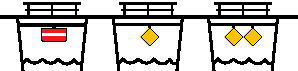
\includegraphics[width=0.7\textwidth]{Hoofdstukken/Bruggen/pdf/brug_vast.pdf}
    \caption{}
    \label{pic:brug:vast}
\end{figure}

\section{Beweegbare bruggen}
Naast vaste bruggen zijn er ook beweegbare bruggen. Deze bruggen hebben lichten in plaats van borden. Vaak heeft een beweegbare brug naast een beweegbare opening, ook een vaste opening. Deze openingen beschikken dan ook over borden of lichten.  

\newpage

% --- Beweegbaar verboden door te varen
\begin{figure}[H]
  \centering
  \begin{minipage}[b]{0.18\textwidth}
    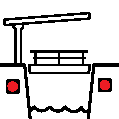
\includegraphics[width=\textwidth]{Hoofdstukken/Bruggen/pdf/brug_doorvaart_verboden.pdf}
    \caption{}
    \label{pic:brug:verboden}
  \end{minipage}
  \hfill
  \begin{minipage}[t]{0.75\textwidth}
  	\vspace{-2.5cm}
    Figuur \ref{pic:brug:verboden} betekent vrijwel hetzelfde als het rode bord uit figuur \ref{pic:brug:vast}. Doorvaart is verboden. Wanneer het echter de enige doorvaart is en je onder de gesloten brug past, mag je er wel door. Er kunnen dan ook tegenliggers aan komen.
  \end{minipage}
\end{figure}
% --- Beweegbaar doorvaart toegestaan, tegenliggende vaart mogelijk
\vspace{-0.75cm}
\begin{figure}[H]
	\centering
	\begin{minipage}[b]{0.18\textwidth}
		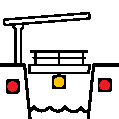
\includegraphics[width=\textwidth]{Hoofdstukken/Bruggen/pdf/brug_doorvaart_toegestaan.pdf}
		\caption{}
		\label{pic:brug:toegestaan}
	\end{minipage}
	\hfill
	\begin{minipage}[t]{0.75\textwidth}
	\vspace{-2.5cm}
	Figuur \ref{pic:brug:toegestaan} heeft de zelfde betekenis als een enkele gele ruit. De doorvaart is toegestaan, maar tegenliggende vaart is mogelijk. Wanneer je de optie hebt, kies dan voor de doorvaart met twee gele lichten. 
\end{minipage}
\end{figure}
% --- Beweegbaar doorvaart toegestaan, tegenliggende vaart niet mogelijk
\vspace{-0.75cm}
\begin{figure}[H]
\centering
\begin{minipage}[b]{0.18\textwidth}
	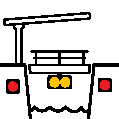
\includegraphics[width=\textwidth]{Hoofdstukken/Bruggen/pdf/brug_doorvaart_geen_tegenligger.pdf}
	\caption{}
	\label{pic:brug:toegestaan_tegenligger}
\end{minipage}
\hfill
\begin{minipage}[t]{0.75\textwidth}
	\vspace{-2.5cm}
	Figuur \ref{pic:brug:toegestaan_tegenligger} staat gelijk aan de twee gele ruiten. De doorvaart is toegestaan en tegenliggende vaart is niet mogelijk. Aan de andere kant van deze brug hangt een enkel rood licht of `verboden in te varen' bord.
\end{minipage}
\end{figure}
% --- Beweegbaar doorvaart aanstonds toegestaan
\vspace{-0.75cm}
\begin{figure}[H]
	\centering
	\begin{minipage}[b]{0.18\textwidth}
		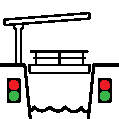
\includegraphics[width=\textwidth]{Hoofdstukken/Bruggen/pdf/brug_aanstonds_toegestaan.pdf}
		\caption{}
		\label{pic:brug:aanstonds}
	\end{minipage}
	\hfill
	\begin{minipage}[t]{0.75\textwidth}
		\vspace{-2.5cm}
		Wanneer je niet onder een brug past en deze beweegbaar is, kan hij voor je opengaan. Wanneer een brug bijna opengaat, gaan de lichten branden als in figuur \ref{pic:brug:aanstonds}. Doorvaart is nog verboden totdat alleen het groene licht brandt
	\end{minipage}
\end{figure}
% --- Beweegbaar doorvaart toegestaan
\vspace{-0.75cm}
\begin{figure}[H]
	\centering
	\begin{minipage}[b]{0.18\textwidth}
		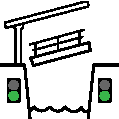
\includegraphics[width=\textwidth,]{Hoofdstukken/Bruggen/pdf/brug_toegestaan.pdf}
		\caption{}
		\label{pic:brug:vrij}
	\end{minipage}
	\hfill
	\begin{minipage}[t]{0.75\textwidth}
		\vspace{-2.5cm}
		Wanneer doorvaart door een beweegbare brug is toegestaan brandt er een enkel groen licht zoals in figuur \ref{pic:brug:vrij}. Het kan ook zijn dat wanneer de brug open is, je eerst een enkel rood licht krijgt. Dit betekent dat de tegenliggers eerst mogen. Hierna zul jij een groen licht krijgen.
	\end{minipage}
\end{figure}
% --- Beweegbaar doorvaart aanstonds verboden
\vspace{-0.75cm}
\begin{figure}[H]
	\centering
	\begin{minipage}[b]{0.18\textwidth}
		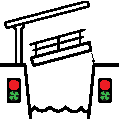
\includegraphics[width=\textwidth]{Hoofdstukken/Bruggen/pdf/brug_sluitend.pdf}
		\caption{}
		\label{pic:brug:sluitend}
	\end{minipage}
	\hfill
	\begin{minipage}[t]{0.75\textwidth}
		\vspace{-2.5cm}
		Wanneer een brug bijna gaat sluiten of aan het sluiten is, gaat er een groen knipperend en rood licht branden, zoals in figuur \ref{pic:brug:sluitend}. De doorvaart is nu verboden, tenzij je redelijkerwijs niet meer kan stoppen. Dit is dus vergelijkbaar met een oranje verkeerslicht. 
	\end{minipage}
\end{figure}
% --- Beweegbaar buiten gebruik
\vspace{-0.75cm}
\begin{figure}[H]
	\centering
	\begin{minipage}[b]{0.18\textwidth}
		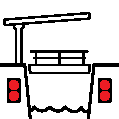
\includegraphics[width=\textwidth]{Hoofdstukken/Bruggen/pdf/brug_buiten_dienst.pdf}
		\caption{}
		\label{pic:brug:buiten}
	\end{minipage}
	\hfill
	\begin{minipage}[t]{0.75\textwidth}
		\vspace{-2.5cm}
		Als er een dubbel rood licht brandt (figuur \ref{pic:brug:buiten}), betekent het dat de brug buiten bediening is. De brugwachter kan dan bijvoorbeeld geen dienst hebben. Doorvaart is dan verboden. Wanneer er echter in het midden één of twee gele ruiten/lichten hangen gelden dezelfde regels als bij een enkel rood licht met gele ruit/licht.
	\end{minipage}
\end{figure}
% --- Beweegbaar gebied
\vspace{-0.75cm}
\begin{figure}[H]
	\centering
	\begin{minipage}[b]{0.18\textwidth}
		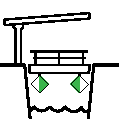
\includegraphics[width=\textwidth,]{Hoofdstukken/Bruggen/pdf/brug_aanbevolen_gebied.pdf}
		\caption{}
		\label{pic:brug:gebied}
	\end{minipage}
	\hfill
	\begin{minipage}[t]{0.75\textwidth}
		\vspace{-2.5cm}
		De ruiten in figuur \ref{pic:brug:gebied} geven iets aan over het aanbevolen vaargebied. Het is aanbevolen om binnen de groene ruiten te blijven varen. Dit kan te maken hebben met bijvoorbeeld een ondiepte of ander obstakel.
	\end{minipage}
\end{figure}
% --- Beweegbaar gebied verbod
\vspace{-0.75cm}
\begin{figure}[H]
\centering
\begin{minipage}[b]{0.18\textwidth}
	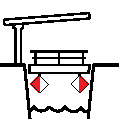
\includegraphics[width=\textwidth]{Hoofdstukken/Bruggen/pdf/brug_verboden_gebied.pdf}
	\caption{}
	\label{pic:brug:gebied_verbod}
\end{minipage}
\hfill
\begin{minipage}[t]{0.75\textwidth}
	\vspace{-2.5cm}
	Soms is het echter ook verboden om in bepaalde gebieden te varen. Dit wordt dan duidelijk gemaakt met de twee rode ruiten in figuur \ref{pic:brug:gebied_verbod}. Je moet dan tussen de rode ruiten in blijven en mag hier niet buiten varen.
\end{minipage}
\end{figure}

% --- Hoogteschaal
\vspace{-0.75cm}
\begin{figure}[H]
	\centering
	\begin{minipage}[b]{0.18\textwidth}
		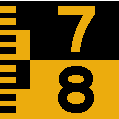
\includegraphics[width=\textwidth]{Hoofdstukken/Reglementen/pdf/hoogteschaal.pdf}
		\caption{}
		\label{pic:brug:schaal}
	\end{minipage}
	\hfill
	\begin{minipage}[t]{0.75\textwidth}
		\vspace{-3cm}
		In sommige gevallen is het bord in figuur \ref{pic:brug:schaal} bij een brug te zien. Deze `hoogteschaal' kan gebruikt worden om de hoogte van de brug tot het water af te lezen. Je leest de hoogte af op het punt waar het water het bord raakt. De hoogte is uitgedrukt in meters.
	\end{minipage}
\end{figure}

\section{Sluizen}
Een sluis wordt gebruikt om een boot te verplaatsen tussen twee wateren met een verschillende hoogte. Wanneer je een sluis in mag varen wordt net als bij bruggen bepaald door lichten.
Bij sluizen hebben de lichten vrijwel exact dezelfde betekenis als bij bruggen. Er zijn echter ook wat kleine verschillen. 

Vaak hangen er in een de sluis zelf ook lichten. Deze maken duidelijk wanneer je de sluis uit mag varen. Wanneer er een sluiswachter aanwezig is moet je goed naar zijn instructies luisteren. Hij geeft vaak aan waar je moet gaan liggen in de sluis. 

% --- Sluis verbod
\hfill
\begin{figure}[H]
	\centering
	\begin{minipage}[b]{0.18\textwidth}
		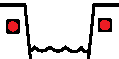
\includegraphics[width=\textwidth]{Hoofdstukken/Bruggen/pdf/sluis_verboden.pdf}
		\caption{}
		\label{pic:sluis:verbod}
	\end{minipage}
	\hfill
	\begin{minipage}[t]{0.75\textwidth}
		\vspace{-2cm}
		Figuur \ref{pic:sluis:verbod} betekent net als bij bruggen dat doorvaart verboden is. Ook als de deuren helemaal open zijn, moet je wachten tot de lichten groen worden. Als er boten in de sluis liggen, moeten deze er namelijk eerst uit.
	\end{minipage}
\end{figure}
% --- Sluis verbod aanstonds
\vspace{-0.35cm}
\begin{figure}[H]
	\centering
	\begin{minipage}[b]{0.18\textwidth}	
		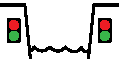
\includegraphics[width=\textwidth]{Hoofdstukken/Bruggen/pdf/sluis_aanstonds.pdf}
		\caption{}
		\label{pic:sluis:aanstonds}
	\end{minipage}
	\hfill
	\begin{minipage}[t]{0.75\textwidth}
		\vspace{-2cm}
		Wanneer de sluis bijna open gaat zullen de lichten aan gaan zoals in figuur \ref{pic:sluis:aanstonds}. Bij sommige sluizen is dit ook te zien als ze bijna gaan sluiten. Je mag er dan alleen nog in varen als je echt niet meer kan stoppen.
	\end{minipage}
\end{figure}
% --- Sluis toegestaan
\vspace{-0.35cm}
\begin{figure}[H]
	\centering
	\begin{minipage}[b]{0.18\textwidth}	
		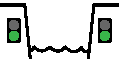
\includegraphics[width=\textwidth]{Hoofdstukken/Bruggen/pdf/sluis_toegestaan.pdf}
		\caption{}
		\label{pic:sluis:toegestaan}
	\end{minipage}
	\hfill
	\begin{minipage}[t]{0.75\textwidth}
		\vspace{-2cm}
		Wanneer je de sluis in mag varen, geeft de sluis een enkel groen licht. Dit is te zien in figuur \ref{pic:sluis:toegestaan}. Wanneer de lichten groen zijn zullen alle boten die eerst in de sluis zaten, deze verlaten hebben. 
	\end{minipage}
\end{figure}
% --- Sluis buiten bedrijf
\vspace{-0.35cm}
\begin{figure}[H]
	\centering
	\begin{minipage}[b]{0.18\textwidth}	
		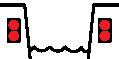
\includegraphics[width=\textwidth]{Hoofdstukken/Bruggen/pdf/sluis_buiten_dienst_dicht.pdf}
		\caption{}
		\label{pic:sluis:buiten}
	\end{minipage}
	\hfill
	\begin{minipage}[t]{0.75\textwidth}
		\vspace{-2cm}
		Een sluis kan net als een brug buiten bedrijf zijn. Dit wordt aangegeven met dubbele rode lichten uit figuur \ref{pic:sluis:buiten}. De deuren zullen in dit geval dicht zijn.
	\end{minipage}
\end{figure}
% --- Sluis buiten toegestaan
\vspace{-0.35cm}
\begin{figure}[H]
	\centering
	\begin{minipage}[b]{0.18\textwidth}	
		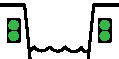
\includegraphics[width=\textwidth]{Hoofdstukken/Bruggen/pdf/sluis_buiten_dienst_open.pdf}
		\caption{}
		\label{pic:sluis:buiten_toegestaan}
	\end{minipage}
	\hfill
	\begin{minipage}[t]{0.75\textwidth}
		\vspace{-2cm}
		Het kan ook voorkomen dat de sluis buiten bedrijf is, maar doorvaart is toegestaan. Beide deuren staan dan open en de sluis geeft een dubbel groen licht, zie figuur \ref{pic:sluis:buiten_toegestaan}
	\end{minipage}
\end{figure}
\paragraph{Spuien en inlaten}
Om aan wachtende schepen de status van de sluis door te geven wordt gebruik gemaakt van een aantal lichten en tekens. Deze tekens zijn optioneel en worden niet door alle sluizen gebruikt. Voor het lozen van water of `spuien' worden de tekens in figuur \ref{pic:sluis:spuien} gebruikt. Het inlaten van water wordt aangegeven met de tekens in figuur \ref{pic:sluis:inlaten}

  \begin{center}
	\begin{minipage}[b]{0.40\textwidth}
		\begin{figure}[H]
			\centering
			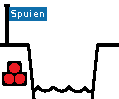
\includegraphics[width=0.46\textwidth]{Hoofdstukken/Bruggen/pdf/sluis_spuien.pdf}
			\caption{Spuien}
			\label{pic:sluis:spuien}
		\end{figure}
	\end{minipage}
	\hspace{1cm}
	\begin{minipage}[b]{0.40\textwidth}
		\begin{figure}[H]
			\centering
			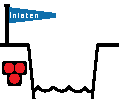
\includegraphics[width=0.46\textwidth]{Hoofdstukken/Bruggen/pdf/sluis_inlaten.pdf}
			\caption{Inlaten}
			\label{pic:sluis:inlaten}
		\end{figure}
	\end{minipage}
\end{center}

\paragraph{Brug en sluis combinatie}
Het komt wel eens voor dat er een sluis en brug direct naast elkaar geplaatst zijn. Let hierbij goed op de lichten. Het kan voorkomen dat je vrij lang voor de open brug moet wachten omdat de sluis eerst leeg moet varen. Wacht dus achter de brug, ook al pas je onder de brug door!

\section{Conclusie}
In dit hoofdstuk zijn alle lichten, tekens en regels voor bruggen en sluizen behandeld. Je weet nu wanneer het verboden en toegestaan is om een brug of sluis door te varen. Deze kennis is bijvoorbeeld heel erg van belang op een hike. Veel van de lichten hebben een logische betekenis en lijken soms zelfs een beetje op verkeerslichten. 
